% main.tex — IJPRAI manuscript, official World Scientific class.
% Class switched from article to ws-ijprai on 2026-08-22 (ijprai-2e.zip,
% extracted 2026-08-22). Converted from draft-v2-full.md.
% Citation keys: all 27 entries in refs.bib verified via arXiv API / CrossRef
% (plan/literature-survey.md, 2026-08-16; arXiv API, 2026-08-21).

\documentclass{ws-ijprai}

\usepackage{xcolor}
\usepackage{url,overcite}
\usepackage[verbose]{hyperref}
\hypersetup{colorlinks=false,allbordercolors=blue,pdfborderstyle={/S/U/W 1}}

\newcommand{\Ldiv}{\mathcal{L}_{\mathrm{div}}}
\newcommand{\etal}{et~al.}

\begin{document}

\markboth{Authors' Names}{Feedback-Controlled Diversity Regularization for Multi-Head Attention}

% Publisher's area — leave empty for submission.
\catchline{}{}{}{}{}

\title{Feedback-Controlled Diversity Regularization for Multi-Head
Attention: Enforcing a Similarity Budget Late in Training}

\author{Author Name} % TODO: real author names (user: leave blank for now)

\address{University Department, University Name, Address\\
City, State ZIP/Zone, Country\\
\email{author\_id@domain\_name}} % TODO: real affiliation/email

\maketitle

\begin{history}
\received{(Day Month Year)}
\revised{(Day Month Year)}
\accepted{(Day Month Year)}
\published{(Day Month Year)}
\end{history}

\begin{abstract}
Multi-head attention tends to learn redundant heads; training-time diversity
penalties reduce them, but their weight is hard to set. A systematic Cora
sweep shows no usable operating point: weights $\le 0.5$ leave inter-head
similarity essentially unchanged (0.95--0.98), while weights $\ge 5$ move it
substantially (0.37--0.67) at a cost of 0.7--2.9 accuracy points, the weakest
weight ($\lambda=5$) doing so at the best checkpoint. We introduce a feedback
controller treating a similarity budget as a set point, adjusting the
regularization weight per epoch via integral control. On three
citation networks with 2-layer GATs (10 seeds), accuracy stays within $\pm
0.4$ points of baseline while the controller meets the budget late in
training on Cora (0.71), approaches it on Citeseer (0.85), and barely on
Pubmed. It beats GradNorm on two of three datasets; linear and Kendall
schedules match it. As a pruning criterion it matches standard criteria, a
null surviving a revival test at late checkpoints, and KD after pruning
recovers $82.00 \pm 0.69$ on Cora, not significantly different from students
trained from scratch with KD at equal budgets, fine-tuning alone leaving a
2.1--2.4 point gap. We claim no accuracy gains from the regularizer or
criterion superiority, on the datasets we test.
\end{abstract}

\keywords{multi-head attention; diversity regularization; feedback control;
head pruning; knowledge distillation; graph attention networks}

\section{Introduction}

Multi-head attention has measurable redundancy. A large fraction of attention
heads can be removed after training with little change in accuracy
\cite{michel2019}, and similarity between attention patterns is a common proxy
for that redundancy~\cite{chai2024}. Two lines of work exploit this
observation. One line prunes or merges heads \emph{after} training using
importance or similarity proxies~\cite{michel2019,voita2019,chai2024,dha2024}.
Another line adds a \emph{training-time} diversity penalty so that heads become
less similar in the first place~\cite{nicolicioiu2023,deacon2024}. Both lines
use fixed hyperparameters: a fixed pruning ratio or a fixed regularization
weight.

In this paper we study the regularization weight itself. Our starting point is
an empirical observation about fixed weights, obtained from a systematic sweep
on Cora (Table~\ref{tab:fixed-lambda}). A diversity penalty that penalizes the
cosine similarity between attention matrices of different heads has two failure
modes, and no intermediate weight escapes them. Weights at or below 0.5 leave
inter-head similarity essentially untouched (0.95--0.98) and $\lambda=1$ moves
it only slightly (0.91); weights at or above 5 do reduce similarity (to
0.37--0.67) but cost about 0.7--2.9 points of test accuracy. The weakest
effective weight ($\lambda=5$) reduces similarity already at the best
checkpoint (0.67), i.e.\ during the accuracy-critical phase. There is no fixed
weight that is both effective and harmless.

This failure spectrum motivates treating the regularization weight as a
\emph{controlled variable} rather than a tuned hyperparameter. We propose a
feedback controller: each epoch, the current inter-head similarity is compared
against a target budget, and the regularization weight is adjusted by an
integral control law. The controller enforces the budget late in training, the
phase where fixed weights are either too weak or too strong, while test
accuracy remains within $\pm 0.4$ points of the unregularized baseline on all
three datasets. The budget is met on Cora (late similarity 0.71), partially
met on Citeseer (0.85), and barely moved on Pubmed within the 200-epoch
budget (Sec.~\ref{sec:h1}); we discuss this dataset dependence explicitly in
Sec.~\ref{sec:limitations}.

Because the regularization signal is itself a redundancy measure, the same
metric can serve as a pruning criterion: after training with the adaptive
regularizer, we score heads by their pairwise similarity to other heads and
keep the least-redundant subset. We then study how this criterion interacts
with fine-tuning and knowledge distillation (KD). We report two findings. First,
KD restores most of the pruning loss (+2.1--2.4 points over fine-tuning alone,
$p=0.001$) and shows no significant difference from small students trained
from scratch with KD at identical budgets: the structured student reaches
the accuracy of the from-scratch student through the pruning path, with no
wall-time saving (Cora; the other two datasets in
Appendix~\ref{app:h3ext}). Second, a strict paired
comparison of pruning criteria (similarity vs.\ gradient, random, and
magnitude) finds no reliable difference among them at GAT scale: 100 epochs of
fine-tuning erase criterion choice. We report this as a negative result,
consistent with the caution in~\cite{michel2019} that criterion quality must be
judged after retraining, not before.

\noindent\textbf{Contributions.}
\begin{arabiclist}
\item A feedback-controlled weighting scheme for head-diversity
  regularization that enforces a similarity budget late in training without
  accuracy loss; the budget is met on Cora, partially met on Citeseer, and
  response-limited on Pubmed; in a regime where no fixed weight is both
  effective and harmless, and against adaptive baselines (linear,
  Kendall-style, and GradNorm schedules; 3 datasets $\times$ 10 seeds; full
  statistics in Sec.~\ref{sec:h1}, Table~\ref{tab:adaptive-baselines}).
\item A structured-compression protocol that reuses the diversity metric as
  the pruning criterion: with KD, pruned students show no significant
  difference from pure-KD students at matched head budgets, and KD recovers
  +2.1--2.4 points over fine-tuning alone ($p=0.001$, Cohen's $d \approx 2.1$;
  Cora in the main text, Citeseer/Pubmed extension in
  Appendix~\ref{app:h3ext}).
\item A strict negative result on pruning-criterion choice at GAT scale
  (paired Wilcoxon signed-rank tests over identical seeds, effect sizes,
  multiplicity discussion), plus a mechanism consistent with the data: at the
  best checkpoint, head similarity is high for every configuration, so the
  similarity signal does not differentiate heads at the point where pruning
  happens. A revival test with criteria computed from late-training
  checkpoints, where the signal is differentiated, reproduces the null
  (Table~\ref{tab:revival}).
\item Reproducible Colab-scale artifacts (T4, $<$100k parameters; protocol,
  seeds, and code at \url{https://github.com/HuKejie/div-prune}).
\end{arabiclist}

\noindent\textbf{Explicit non-claims.} We do not claim that the regularizer
\emph{improves} accuracy (it is no-harm only); we do not claim that the
diversity criterion is better than existing pruning criteria (the contrast is
null); we do not claim that pruning+KD \emph{beats} pure KD (no significant
difference is detectable, Sec.~\ref{sec:h3}). All evidence is at GAT scale on
three citation networks; transfer to other architectures is untested.

\section{Related Work}
\label{sec:related}

\textbf{Head redundancy and pruning.} The redundancy of multi-head attention is
well documented.~\cite{michel2019} shows that many heads can be removed with
little loss and proposes a greedy, gradient-based head-importance criterion,
cautioning that pruning without retraining misrepresents criterion quality.
\cite{voita2019} learns L0 gates during training to prune heads. At LLM scale,
similarity between attention patterns is exploited for inference-time head
clustering and fusion: CHAI clusters correlated heads~\cite{chai2024}, DHA
fuses similar key/value heads~\cite{dha2024}, and ProxyAttn approximates
attention with representative heads~\cite{proxyattn2025}. These works use head
similarity \emph{after} training; none uses it as a training-time
regularization signal. Note the scale gap: that evidence is at LLM scale,
while all experiments in this paper are at 92k-parameter GAT scale on three
citation networks (Sec.~\ref{sec:limitations}).

\textbf{Diversity regularization for attention.} Training-time diversity
penalties exist in several forms: HSIC or orthogonality regularizers on head
subspaces~\cite{yun2021}, diversity-promoting losses for ASR conformers
\cite{audhkhasi2022}, multi-level redundancy reduction for ViTs
\cite{chen2022}, and orthogonalization of head input gradients
\cite{nicolicioiu2023}. DEACON trains a GHA-based projection so that heads
occupy a maximum-variance subspace and then prunes heads with the same PCA
criterion~\cite{deacon2024}, the closest work coupling diversity-enforcing
training with same-criterion pruning. It differs from ours in criterion (PCA
variance vs.\ pairwise cosine similarity), in weighting (fixed vs.\
feedback-controlled), and in scope (no GNN coverage, no distillation).
\cite{jhareagen2025} adapts the strength of an entropy-based diversity
regularizer per head for private inference; to our knowledge no prior work
applies feedback control to the global weight of a diversity loss.

\textbf{Adaptive loss weighting.} Learning or scheduling loss weights is
standard in multi-task learning: homoscedastic uncertainty weighting
\cite{kendall2018}, gradient normalization~\cite{gradnorm2018}, and excess-risk
weighting~\cite{excessmtl2024}.~\cite{harvey2024} learns the strength of a
regularization term in a variational fine-tuning setting. These mechanisms
target task or regularization balance; none is applied to head-diversity
regularization.

\textbf{KD and GNN compression.} KD~\cite{hinton2015} compresses models by
matching student outputs to teacher outputs. For transformers, TinyBERT and
MiniLM distill attention-level information~\cite{tinybert2020,minilm2020}; for
GNNs, GLNN distills a GNN teacher into an MLP student~\cite{glnn2022} and KRD
shows reliability-weighted distillation can exceed the teacher~\cite{krd2023}.
Pruning-before-distillation pipelines exist~\cite{parkno2021,epsd2024,ddk2024},
but none couples a diversity criterion with distillation. Our closest
comparison is pure KD at matched budgets (Sec.~\ref{sec:h3}); omitting it
would leave open the possibility that KD alone already captures the benefit.

\noindent\textbf{Positioning.} The combination we study, (a) the same
similarity metric used for training-time regularization and for pruning, (b) a
feedback-controlled regularization weight, and (c) distillation, at small-model
scale (GAT, $\leq$100k parameters), is, to our knowledge, unoccupied. The
nearest neighbors are DEACON~\cite{deacon2024} (shared criterion, fixed
weights, no KD) and Nicolicioiu \etal{}~\cite{nicolicioiu2023} (regularize then
prune, but the pruning signal is OOD attribution, not the diversity metric).

\section{Method}

\subsection{Setup and diversity regularization}

We use a standard 2-layer GAT~\cite{velickovic2018} with 8 heads and hidden
size 8 per head (92{,}373 parameters) on the Planetoid citation networks Cora,
Citeseer, Pubmed~\cite{yang2016}. Let $A_h^{(l)}$ denote the attention matrix
of head $h$ in layer $l$ (softmax-normalized attention coefficients). The
diversity loss penalizes the mean pairwise cosine similarity between attention
matrices of different heads in the same layer:
\begin{equation}
\Ldiv \;=\; \frac{2}{H(H-1)} \sum_{l} \sum_{h<k}
\cos\!\big(A_h^{(l)},\, A_k^{(l)}\big).
\label{eq:ldiv}
\end{equation}
The training objective is $L = L_{\mathrm{CE}} + \lambda \Ldiv$, where
$L_{\mathrm{CE}}$ is the cross-entropy loss. This is the attention-level
variant; an output-level variant (Euclidean distance between head outputs)
exists but is not used in the main experiments.

\subsection{The fixed-$\lambda$ failure spectrum}

Sweeping $\lambda$ on Cora (Table~\ref{tab:fixed-lambda}) shows two failure
modes. For $\lambda \le 0.5$, the penalty is too weak to move similarity:
inter-head similarity stays at 0.95--0.98, indistinguishable from
unregularized training, and $\lambda=1$ moves it only slightly (0.91). For
$\lambda \ge 5$, similarity drops (0.37--0.67 at
the best checkpoint) but test accuracy degrades by about 0.7--2.9 points. The
weakest effective weight, $\lambda=5$, already reaches 0.67 \emph{at the best
checkpoint}: it enforces diversity during the accuracy-critical phase,
which is the timing failure we attribute to GradNorm in
Sec.~\ref{sec:h1}. No fixed weight is simultaneously effective and harmless.

\subsection{Feedback-controlled adaptive $\lambda$}

We treat the target similarity budget $d^*$ as a set point and $\lambda$ as the
control variable. Each epoch $t$, we compute the current similarity $d_t$ (the
same quantity as in Eq.~\eqref{eq:ldiv}, averaged over the training set) and
update
\begin{equation}
\lambda_{t+1} \;=\; \mathrm{clamp}_{[0,\,\lambda_{\max}]}\!\big(\lambda_t +
\eta\,(d_t - d^*)\big),
\label{eq:control}
\end{equation}
starting from $\lambda_0 = 0$, with target $d^* = 0.7$, gain $\eta = 0.05$, and
ceiling $\lambda_{\max} = 3.0$, held constant across all three datasets. The
integral law accumulates error only while $d_t$ exceeds the budget, so
$\lambda$ winds up when similarity is high and stops changing once the budget
is met. No $\lambda$ is set by hand: the same three constants
$(d^*, \eta, \lambda_{\max})$ are used everywhere. The three constants were
chosen once on Cora and never re-tuned: $d^*=0.7$ sits just above the
similarities the fixed sweep reaches (0.37--0.67) and far below the
unregularized level ($\sim$0.97); $\eta=0.05$ gives a per-epoch weight
increment of $\eta\,(d_t-d^*) \approx 0.015$ at the unregularized similarity,
so the weight builds up over the $\sim$100-epoch late phase rather than
overshooting within a few epochs; and $\lambda_{\max}=3.0$ sits below the
regime ($\lambda \ge 5$) where fixed weights become harmful
(Sec.~\ref{sec:spectrum}). A sensitivity grid over $(\eta, d^*)$ is reported
in Appendix~\ref{app:sens}. The ceiling is a stability
guard, not an operating point: $\lambda$ converges below it on every run
(final values 0.27--1.94 per dataset at the chosen gain; a $4\times$-gain
probe on Pubmed saturates the ceiling, Sec.~\ref{sec:h1}). The update is cheap (one
forward-pass statistic per epoch) and adds no parameters.

\subsection{Pruning with the diversity criterion}

After training with the adaptive regularizer, the diversity metric doubles as a
pruning criterion. For each head, we compute its mean pairwise cosine
similarity to all other heads in the same layer (over the training set); heads
with the lowest similarity are the least redundant and are kept. The pruning
protocol follows the structure of~\cite{michel2019}: equal fractions per layer,
at least one head per layer kept, with prune ratios 0.5 and 0.75 (keeping 4/8
and 2/8 heads). Baselines are gradient-based importance~\cite{michel2019},
random selection, and magnitude ($L_2$ norm of head weights). The criterion is
scored at a checkpoint of the trained teacher: the early-stopping best
checkpoint, the lowest-similarity checkpoint, or the final checkpoint; the
main results use the best checkpoint (the revival test across sources is
reported in Sec.~\ref{sec:h2}). Pruned models are then fine-tuned for a fixed
100 epochs.

\subsection{KD pipeline}

For the compression study, the pruned student is trained by logit KD from the
dense adaptive teacher: $L = (1-\alpha)\,L_{\mathrm{CE}} + \alpha\, T^2\,
L_{\mathrm{KL}}$, with $\alpha = 0.5$ and $T = 2$, for 100 epochs, the same
epoch budget as the pure-KD comparison (students trained from scratch with KD).
All comparisons are at matched head budgets (4/8 or 2/8 heads) so that the
accuracy--parameter trade-off, not the training recipe, is the variable.
Because both GAT layers shrink with the head count (layer 1 per-head
attention weights, layer 2 concatenation input), matched head budgets also
match parameter counts: 92{,}373 parameters at 8/8 heads, 46{,}197 at 4/8, and
23{,}109 at 2/8. In addition to the three arms B5/B6/B8 (pure KD, prune +
fine-tuning, prune + KD), we report B4: small models trained from scratch at
the same budgets with plain cross-entropy and no distillation, the
reference that tells us whether the pruning path loses anything relative to
simply training small.

\section{Experiments}

\noindent\textbf{Setup and statistics.} GAT 2-layer, 8 heads, hidden 8/head
(92{,}373 parameters), Adam optimizer (learning rate 0.005, weight decay
$5{\times}10^{-4}$), dropout 0.6, fixed Planetoid split, early stopping with
patience 100 (max 200 epochs), fine-tuning and KD for 100 epochs. 10 seeds per
configuration. Results are mean $\pm$ std over seeds; 95\% CIs are in the
appendix (Table~\ref{tab:ci} and Table~\ref{tab:revision-cis}). Comparisons
use paired Wilcoxon signed-rank tests over identical
seeds: one-sided where a direction is hypothesized, two-sided with 95\% CIs
on the difference for tie claims; where tied pairs occur, the normal
approximation is used and the paired $t$-test is reported alongside. Effect
sizes (Cohen's $d$) are reported for major contrasts. Compute: Google Colab
T4; each dense run takes seconds at this scale (wall times in
Sec.~\ref{sec:h3}). The revision experiments (adaptive baselines, controller
checkpoints, the revival matrix, and the H3 extension) were executed from a
versioned Colab notebook with per-combination progress logging; merged
results and teacher checkpoints are archived (Sec.~\ref{sec:limitations}).
The second-revision experiments ($\lambda=5$ comparisons and the controller
sensitivity grid) were executed locally with the same Hydra pipeline and
identical configs; their CSV results are archived with the same layout.

\subsection{Can fixed $\lambda$ control diversity?}
\label{sec:spectrum}

\emph{Claim tested: no fixed weight is simultaneously effective and harmless.}

Table~\ref{tab:fixed-lambda} (top) reports the Cora sweep. The answer is no:
$\lambda \le 0.5$ leaves similarity at 0.95--0.98 and $\lambda=1$ moves it
only slightly (0.91); $\lambda \ge 5$ moves it but costs about 0.7--2.9
points. Note where $\lambda=5$ moves it: at the best
checkpoint (0.67), not late in training, the timing failure analyzed in
Sec.~\ref{sec:h1}. This is the motivation for feedback control.

% Table 1: fixed-lambda failure spectrum (Cora) + H1 main comparison.
% WS-IJPRAI table format (caption above via \tbl). Numbers: stats-appendix.md
% (updated 2026-09-08), results_clean.csv + outputs_rev2_sweep.
\begin{table}[th]
\tbl{Fixed-$\lambda$ failure spectrum on Cora (top) and the main comparison of
training configurations across three citation networks (bottom). Accuracy is
mean~$\pm$~std over seeds. Top: second-revision re-run at $n{=}10$ per weight
with recorded similarities, which supersedes the pre-submission $n{=}5$ sweep.
Bottom: $n{=}10$; the Cora fixed-$\lambda{=}20$ cell uses the second-revision
batch, Citeseer and Pubmed use the original batch (identical protocol).
$d_{\mathrm{best}}$ is the inter-head similarity at the best checkpoint.
\label{tab:fixed-lambda}}
{\begin{tabular}{lccc}
\toprule
\multicolumn{3}{c}{\textbf{Fixed-$\lambda$ sweep, Cora (attention-level)}} & \\
\colrule
$\lambda$ & Test acc.\ (\%) & $d_{\mathrm{best}}$ & \\
\colrule
0.01 & $81.16 \pm 1.63$ & 0.979 & \\
0.1  & $81.03 \pm 1.50$ & 0.978 & \\
0.5  & $81.13 \pm 1.37$ & 0.954 & \\
1.0  & $81.08 \pm 1.68$ & 0.906 & \\
5.0  & $80.50 \pm 1.44$ & 0.674 & \\
20.0 & $79.71 \pm 1.24$ & 0.597 & \\
50.0 & $78.22 \pm 1.88$ & 0.366 & \\
\colrule
\multicolumn{4}{c}{\textbf{Main comparison (10 seeds per cell)}} \\
\colrule
Dataset & Baseline & Fixed $\lambda{=}20$ & Adaptive ($t{=}0.7$, $\eta{=}0.05$) \\
\colrule
Cora     & $81.15 \pm 1.02$ & $79.71 \pm 1.24$ & $80.79 \pm 0.92$ \\
Citeseer & $68.27 \pm 1.56$ & $66.55 \pm 2.00$ & $68.46 \pm 1.35$ \\
Pubmed   & $77.52 \pm 0.54$ & $76.30 \pm 0.68$ & $77.44 \pm 0.67$ \\
\botrule
\end{tabular}}
\end{table}


\subsection{Adaptive $\lambda$ vs.\ fixed $\lambda$ vs.\ baseline}
\label{sec:h1}

\emph{Claim tested: the controller enforces the budget without accuracy loss
where fixed $\lambda$ fails.}

Table~\ref{tab:fixed-lambda} (bottom) and Fig.~\ref{fig:h1} compare baseline,
fixed $\lambda=20$, and adaptive ($t=0.7$, $\eta=0.05$) on all three datasets
(fixed $\lambda=5$ is examined through the sweep above).
Adaptive $\lambda$ keeps accuracy within $\pm 0.4$ points of baseline
everywhere (Cora $80.79 \pm 0.92$ vs.\ $81.15 \pm 1.02$; Citeseer $68.46 \pm
1.35$ vs.\ $68.27 \pm 1.56$; Pubmed $77.44 \pm 0.67$ vs.\ $77.52 \pm 0.54$);
all CIs overlap. Fixed $\lambda=20$ is below both everywhere ($-1.1$ to
$-1.9$). Fixed $\lambda=5$, the strongest fixed weight in the sweep,
costs about 0.7 points on Cora and moves similarity at the best checkpoint
(details in Table~\ref{tab:fixed-lambda}): it belongs to the same timing
quadrant as GradNorm (below). The controller converges to different final
weights per dataset (Cora
$\lambda_{\mathrm{final}}=0.84$, Citeseer 0.27, Pubmed 1.94), which is the
point: the controller finds the per-dataset operating point that a fixed sweep
cannot.

\begin{figure}[t]
\centerline{
\includegraphics[width=5in]{figures/fig1_h1_comparison.pdf}}
\caption{Test accuracy of a 2-layer GAT on three citation networks under
baseline training, fixed-$\lambda$ ($\lambda=20$) diversity regularization,
and feedback-controlled adaptive regularization (target 0.7, $\eta=0.05$).
Bars are means over 10 seeds; error bars are $\pm$1 standard deviation over
seeds; values above bars are means. The adaptive configuration stays within
$\pm$0.4 points of baseline on all three datasets; no fixed weight achieves
both an effect on similarity and this level of accuracy (see
Table~\ref{tab:fixed-lambda}).}
\label{fig:h1}
\alttext{Grouped bar chart of test accuracy for baseline, fixed-lambda, and
adaptive configurations on Cora, Citeseer, and Pubmed.}
\end{figure}

\noindent\textbf{Mechanism (Fig.~\ref{fig:trace}).} Training traces show the
closed loop working: similarity falls from $\sim$0.995 toward the 0.7 budget as
the integral controller raises $\lambda$, while validation accuracy stays flat.
The divergence is enforced \emph{late} in training, after the best checkpoint
is selected: the best-checkpoint similarity therefore remains high (Cora
0.934; Citeseer 0.988; Pubmed 0.996). We emphasize this distinction
throughout: the controller enforces the budget late in training; it does not
claim to reduce similarity at the selected checkpoint. How far the late phase
gets is dataset-dependent: on Cora the budget is met (late similarity 0.706);
on Citeseer similarity moves substantially toward it (0.847); on Pubmed it
barely moves (0.988). A second-revision probe quadrupled the gain
($\eta=0.2$, nine seeds): the weight saturates at the 3.0 ceiling, yet late
similarity still barely moves (0.993). The Pubmed run is thus
\emph{response-limited}: its similarity responds too slowly to the penalty at
any weight within the configured ceiling, so more gain does not buy the
budget there (Appendix~\ref{app:sens}).

\begin{figure}[t]
\centerline{
\includegraphics[width=5in]{figures/fig2_trace_cora_seed3.pdf}}
\caption{Adaptive-controller dynamics on Cora, seed 3 (same-protocol run; see
Sec.~\ref{sec:limitations} for the provenance note): (a) head similarity $d_t$
falls toward the 0.7 budget as (b) the integral controller raises $\lambda$;
(c) validation accuracy remains flat. The budget is enforced late in training,
after the best checkpoint is selected.}
\label{fig:trace}
\alttext{Three-panel line plot of head similarity, controller lambda, and
validation accuracy over training epochs on Cora.}
\end{figure}

\noindent\textbf{Adaptive baselines (Table~\ref{tab:adaptive-baselines},
Fig.~\ref{fig:baselines}).} A controller that beats only fixed weights invites
the question whether any adaptive scheme would do. We compare the controller
against three adaptive baselines on all datasets (10 paired seeds): an
open-loop linear ramp calibrated to the controller's slope on Cora and
transferred unchanged, Kendall--Gal uncertainty weighting~\cite{kendall2018},
and GradNorm~\cite{gradnorm2018}. The controller matches the linear and
Kendall-style schedules on accuracy everywhere ($|\Delta| \le 0.48$~pp; no
contrast is significant under one-sided paired tests) and beats GradNorm
significantly on Cora ($+1.75$~pp, $p=0.010$) and Pubmed ($+1.37$~pp,
$p=0.005$; Citeseer $+1.10$~pp, $p=0.053$).
The difference is timing. GradNorm is the only baseline whose best-checkpoint
similarity reaches the 0.7 budget ($d_{\mathrm{best}}=0.69$ on Cora and
Citeseer): it diverges heads during the accuracy-critical phase while its
weight saturates at the renormalization bound
($\lambda_{\mathrm{final}}\approx1.95$ on every dataset; on Pubmed it
saturates without moving similarity at all). The linear and Kendall schedules
do not enforce the budget at the best checkpoint ($d_{\mathrm{best}} \ge
0.849$ everywhere) and stay harmless. On Cora, the controller enforces the
budget late, after the best checkpoint, while matching baseline accuracy.
Late-phase similarity was logged only for the controller; the baselines'
timing is therefore judged by best-checkpoint similarity alone, a protocol
limitation we state in Sec.~\ref{sec:limitations}.

\noindent\textbf{Baseline adaptations.} GradNorm is designed for multi-task
balance; we use its two-term form with the CE loss and $\Ldiv$ as the two
``tasks'': each epoch, the gradient norms of both terms with respect to the
shared weights are measured, and the divergence weight is nudged toward
equalizing the normalized norms (asymmetry $\alpha=0$, step $\eta=0.16$);
both weights are then renormalized to sum to 2. The saturation at
$\lambda\approx1.95$ follows from the combination of a 0.05 floor on the CE
weight with the sum-to-2 renormalization, which bounds the divergence weight
at $2-0.05=1.95$. The Kendall--Gal baseline treats $\Ldiv$ as a second
``task'' with a learnable log-variance: $L = e^{-s_{\mathrm{CE}}}L_{\mathrm{CE}}
+ e^{-s_{\mathrm{div}}}\Ldiv + (s_{\mathrm{CE}}+s_{\mathrm{div}})/2$, and we
report the effective weight $\lambda = e^{-s_{\mathrm{div}}}$.

\begin{figure}[t]
\centerline{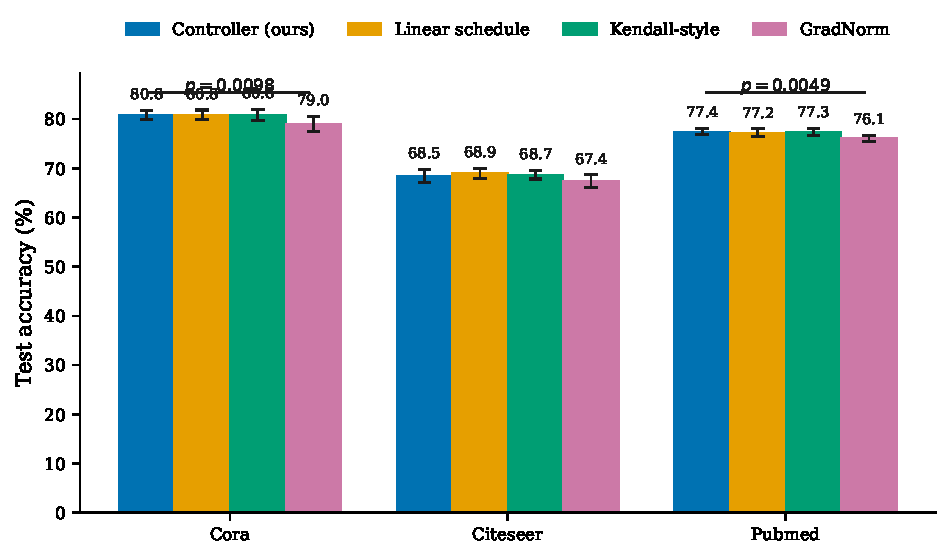
\includegraphics[width=5in]{figures/fig4_adaptive_baselines.pdf}}
\caption{Controller vs.\ adaptive baselines on three citation networks. Bars
are means over 10 seeds; error bars are $\pm$1 standard deviation. Brackets:
one-sided paired Wilcoxon signed-rank tests, controller vs.\ GradNorm,
$p=0.010$ (Cora) and $p=0.005$ (Pubmed); Citeseer $p=0.053$. Linear and
Kendall schedules match the controller on accuracy but do not enforce the
budget at the best checkpoint; GradNorm enforces it already at the best
checkpoint and pays 1.1--1.8 points. The controller enforces the budget late
in training without accuracy loss; late-phase similarity was not logged for
the three baselines (Table~\ref{tab:adaptive-baselines}).}
\label{fig:baselines}
\alttext{Grouped bar chart of test accuracy for the controller, linear,
Kendall-style, and GradNorm schedules on Cora, Citeseer, and Pubmed.}
\end{figure}

% Table (number assigned by position): adaptive-baseline comparison
% (M1 revision, Colab batch B1). WS-IJPRAI table format. Numbers:
% stats-appendix.md R1 (2026-09-06). Controller rows: submitted dense
% adaptive block (distill=False), n=10 per dataset.
\begin{table}[th]
\tbl{Controller vs.\ adaptive baselines (one-sided paired tests, 10 seeds). Accuracy is mean~$\pm$~std per cell; $\lambda_{\mathrm{final}}$ and $d_{\mathrm{best}}$ are the mean final controller weight and the inter-head similarity at the best checkpoint. GradNorm is the only baseline whose best-checkpoint similarity reaches the budget, at a significant accuracy cost; linear and Kendall schedules stay accuracy-neutral and do not enforce the budget at the best checkpoint. The controller enforces the budget late in training while matching baseline accuracy (late-phase similarity was not logged for the three baselines).
\label{tab:adaptive-baselines}}
{\begin{tabular}{llccccc}
\toprule
Dataset & Schedule & Test acc.\ (\%) & $\lambda_{\mathrm{final}}$ & $d_{\mathrm{best}}$ & $\Delta$ vs.\ ctrl.\ (pp) & $p$ (paired) \\
\colrule
Cora & Controller & $80.79 \pm 0.92$ & 0.84 & 0.934 & --- & --- \\
 & Linear & $80.83 \pm 1.05$ & 0.87 & 0.924 & $-0.04$ & 0.4531 \\
 & Kendall & $80.83 \pm 1.21$ & 1.37 & 0.849 & $-0.04$ & 0.5781 \\
 & Gradnorm & $79.04 \pm 1.57$ & 1.95 & 0.693 & $+1.75$ & 0.0098 \\
\colrule
Citeseer & Controller & $68.46 \pm 1.35$ & 0.27 & 0.988 & --- & --- \\
 & Linear & $68.94 \pm 1.01$ & 0.30 & 0.976 & $-0.48$ & 0.7764 \\
 & Kendall & $68.66 \pm 0.90$ & 1.10 & 0.969 & $-0.20$ & 0.6055 \\
 & Gradnorm & $67.36 \pm 1.35$ & 1.95 & 0.688 & $+1.10$ & 0.0527 \\
\colrule
Pubmed & Controller & $77.44 \pm 0.67$ & 1.94 & 0.996 & --- & --- \\
 & Linear & $77.23 \pm 0.79$ & 1.67 & 0.995 & $+0.21$ & 0.3477 \\
 & Kendall & $77.32 \pm 0.76$ & 1.26 & 0.996 & $+0.12$ & 0.3389 \\
 & Gradnorm & $76.07 \pm 0.67$ & 1.95 & 1.000 & $+1.37$ & 0.0049 \\
\colrule
\botrule
\end{tabular}}
\end{table}


\subsection{Does the diversity criterion beat standard pruning criteria?}
\label{sec:h2}

\emph{Claim tested: the $\Ldiv$ similarity signal selects better heads than
gradient/random/magnitude.}

Under adaptive teachers at prune ratio 0.75 (10 paired seeds, fine-tuning 100
epochs, no KD), all contrasts are null: vs.\ random $+0.05$~pp (one-sided
Wilcoxon $p=0.28$), vs.\ gradient $-0.13$~pp ($p=0.63$), vs.\ magnitude
$+0.01$~pp ($p=0.54$). At ratio 0.5 and under B0 (unregularized) teachers the
pattern
repeats: of the nine remaining cells (Adaptive ratio 0.5 and B0 ratios 0.5
and 0.75, three criteria each), eight have one-sided Wilcoxon
$p=0.50$--$1.00$, with one exception: under the B0 teacher at ratio 0.5,
diversity vs.\ gradient shows $+0.62$~pp (Wilcoxon $p=0.094$, paired-$t$
$p=0.048$, $d=0.97$). This does not survive multiplicity control
(Holm--Bonferroni across the 12 contrasts: the smallest $p$-value, 0.048, is
above the corrected threshold $0.05/12 \approx 0.0042$, so no contrast
survives) and is directionally inconsistent with the main comparison. The ratio-0.5 and
B0-teacher cells come from the pre-submission batch and use $n=5$ seeds per
arm (5 pairs); the adaptive-teacher ratio-0.75 contrasts use the 10-seed
revision batch. We report
the full matrix in Table~\ref{tab:criteria} and conclude: at GAT scale with
100-epoch fine-tuning, the similarity criterion performs on par with strong
baselines, and we find no evidence that it is better.

% Table (number assigned by position): pruning-criterion contrasts (H2).
% Regenerated 2026-09-06 from results_clean.csv. Adaptive-teacher ratio-0.75
% rows use the B3 `best`-source runs (supersede the pre-merge rows dropped
% in the 2026-09-05 merge; see stats-appendix.md H2 note).
\begin{table}[th]
\tbl{Paired comparison of pruning criteria at GAT scale (fine-tuning 100 epochs, no KD; identical seeds within each contrast). $\Delta$ is the accuracy difference (diversity criterion minus baseline criterion) in percentage points; Cohen's $d$ is reported for each contrast. Wilcoxon $p$-values are one-sided (diversity $>$ baseline). No contrast survives multiplicity control (Holm--Bonferroni across the 12 tests); the single nominally significant pair (B0 teacher, ratio 0.5, vs.\ gradient) rests on 5 pairs (these pre-submission cells use $n{=}5$ seeds per arm; the adaptive-teacher ratio-0.75 cells use the 10-seed revision batch) and is directionally inconsistent with the main comparison. Tied pairs in the Wilcoxon test fall back to the normal approximation; paired-$t$ $p$-values are reported alongside.
\label{tab:criteria}}
{\begin{tabular}{lllcccc}
\toprule
Teacher & Ratio & Contrast & $\Delta$ (pp) & Wilcoxon $p$ & Paired-$t$ $p$ & $d$ \\
\colrule
Adaptive & 0.5 & div vs.\ random & $-1.20$ & 1.0000 & 0.9828 & -1.41 \\
Adaptive & 0.5 & div vs.\ gradient & $-0.22$ & 0.7812 & 0.6893 & -0.24 \\
Adaptive & 0.5 & div vs.\ magnitude & $-0.26$ & 0.8125 & 0.7677 & -0.36 \\
Adaptive & 0.75 & div vs.\ random & $+0.05$ & 0.2783 & 0.4466 & +0.04 \\
Adaptive & 0.75 & div vs.\ gradient & $-0.13$ & 0.6289 & 0.7593 & -0.23 \\
Adaptive & 0.75 & div vs.\ magnitude & $+0.01$ & 0.5391 & 0.4807 & +0.02 \\
B0 & 0.5 & div vs.\ random & $-0.34$ & 0.7812 & 0.8067 & -0.43 \\
B0 & 0.5 & div vs.\ gradient & $+0.62$ & 0.0938 & 0.0485 & +0.97 \\
B0 & 0.5 & div vs.\ magnitude & $-0.20$ & 0.5938 & 0.6924 & -0.24 \\
B0 & 0.75 & div vs.\ random & $-0.48$ & 0.9062 & 0.8254 & -0.47 \\
B0 & 0.75 & div vs.\ gradient & $+0.04$ & 0.5000 & 0.4778 & +0.03 \\
B0 & 0.75 & div vs.\ magnitude & $+0.12$ & 0.6875 & 0.4110 & +0.11 \\
\botrule
\end{tabular}}
\end{table}


\noindent\textbf{Mechanism.} The criterion is computed at the best checkpoint,
where head similarity is high for every configuration (0.93--0.99). At the
point where pruning happens, the $\Ldiv$ signal does not differentiate heads.
This is consistent with~\cite{michel2019}: fine-tuning washes out criterion
choice.

\noindent\textbf{Revival test (Table~\ref{tab:revival}).} The negative result
could be an artifact of this timing: the controller moves similarity late in
training (Sec.~\ref{sec:h1}), so a criterion computed at a late checkpoint
might recover the signal. We therefore pruned from three checkpoint sources
(best, lowest-similarity, final) with all four criteria, 10 seeds per cell, on
all datasets (prune ratio 0.75, fine-tuning 100 epochs, no KD). The
lowest-similarity checkpoint coincides with the final one in 119 of 120
combinations, since similarity decreases monotonically under the controller,
so the late source carries the differentiated signal ($d_{\mathrm{src}} =
0.71$--$0.85$ on Cora and Citeseer). All nine late-source contrasts remain
null (one-sided $p \ge 0.078$; the nominally largest effect favors random,
$-0.87$~pp on Pubmed), and pruning from the best checkpoint is never
significantly worse than pruning from the late one; on Citeseer the best
checkpoint is significantly better ($+1.90$~pp, $p=0.001$). The negative
criterion result is therefore not a timing artifact: even where the $\Ldiv$
signal differentiates heads, 100 epochs of fine-tuning erase criterion
choice. On Pubmed the probe is weak: the teacher's late similarity stays
at 0.99, because the run is response-limited there (Sec.~\ref{sec:h1}
shows even a $4\times$ gain saturates the ceiling without moving
similarity), so the decisive evidence is Cora and Citeseer.

% Table (number assigned by position): revival test (M2 revision, Colab
% batches B2/B3). WS-IJPRAI table format. Numbers: stats-appendix.md R2
% (2026-09-06). Prune ratio 0.75, controller teacher, FT 100 epochs, no KD,
% 10 seeds per cell.
\begin{table}[th]
\tbl{Revival test: pruning criteria computed from late-training checkpoints. Top: test accuracy (mean~$\pm$~std) by checkpoint source and criterion. $d_{src}$ is the teacher's head similarity at the checkpoint source. The lowest-similarity checkpoint coincides with the final one in 119/120 (dataset, seed, criterion) combinations (similarity decreases monotonically), so $d_{src}$ for the late source is the teacher's final similarity. Bottom: one-sided paired contrasts (diversity vs.\ baseline criterion) at the late source, the timing where the signal is actually differentiated; none is significant, and the nominally largest effect favors random. The negative criterion result therefore survives the revival test.
\label{tab:revival}}
{\begin{tabular}{llcccccc}
\toprule
Dataset & Source & $d_{src}$ & & Diversity & Magnitude & Gradient & Random \\
\colrule
Cora & Best & 0.934 & & $80.32 \pm 0.78$ & $80.31 \pm 0.59$ & $80.45 \pm 0.66$ & $80.27 \pm 0.75$ \\
 & Late (min div.) & 0.706 & & $80.36 \pm 1.49$ & $79.95 \pm 0.86$ & $79.88 \pm 1.01$ & $79.74 \pm 1.05$ \\
 & Late (last) & 0.706 & & $80.36 \pm 1.49$ & $79.95 \pm 0.86$ & $79.88 \pm 1.01$ & $79.74 \pm 1.05$ \\
\colrule
Citeseer & Best & 0.972 & & $67.95 \pm 1.17$ & $67.94 \pm 1.13$ & $67.77 \pm 1.36$ & $68.35 \pm 1.05$ \\
 & Late (min div.) & 0.847 & & $66.05 \pm 1.35$ & $66.21 \pm 1.80$ & $66.65 \pm 1.67$ & $66.87 \pm 1.19$ \\
 & Late (last) & 0.847 & & $66.05 \pm 1.35$ & $66.18 \pm 1.86$ & $66.65 \pm 1.67$ & $66.87 \pm 1.19$ \\
\colrule
Pubmed & Best & 0.995 & & $76.35 \pm 0.93$ & $76.33 \pm 1.02$ & $77.02 \pm 0.72$ & $76.77 \pm 1.51$ \\
 & Late (min div.) & 0.988 & & $76.17 \pm 1.25$ & $75.98 \pm 1.03$ & $76.51 \pm 0.76$ & $77.04 \pm 1.31$ \\
 & Late (last) & 0.988 & & $76.17 \pm 1.25$ & $75.98 \pm 1.03$ & $76.51 \pm 0.76$ & $77.04 \pm 1.31$ \\
\colrule
\multicolumn{8}{l}{\textbf{Paired contrasts at the late source (diversity minus baseline, 10 pairs)}} \\
\colrule
Dataset & Contrast & $\Delta$ (pp) & & Wilcoxon $p$ & Paired-$t$ $p$ & $d$ & \\
\colrule
Cora & vs.\ random & $+0.62$ & & 0.1162 & 0.1153 & 0.41 & \\
Cora & vs.\ magnitude & $+0.41$ & & 0.0781 & 0.0779 & 0.49 & \\
Cora & vs.\ gradient & $+0.48$ & & 0.1436 & 0.1223 & 0.39 & \\
Citeseer & vs.\ random & $-0.82$ & & 0.9502 & 0.9475 & -0.57 & \\
Citeseer & vs.\ magnitude & $-0.16$ & & 0.6289 & 0.6122 & -0.09 & \\
Citeseer & vs.\ gradient & $-0.60$ & & 0.8691 & 0.8296 & -0.32 & \\
Pubmed & vs.\ random & $-0.87$ & & 0.9756 & 0.9589 & -0.62 & \\
Pubmed & vs.\ magnitude & $+0.19$ & & 0.2656 & 0.1509 & 0.35 & \\
Pubmed & vs.\ gradient & $-0.34$ & & 0.8203 & 0.8391 & -0.33 & \\
\botrule
\end{tabular}}
\end{table}


\subsection{Does KD recover pruning loss, and how does prune+KD compare to pure KD?}
\label{sec:h3}

\emph{Claim tested: KD restores pruned-model accuracy; against pure KD at the
same head budget, no significant difference is detectable.}

At both budgets, KD recovers most of the pruning loss: B8 (prune+KD) vs.\ B6
(prune+FT) gains $+2.11$~pp at 4/8 heads and $+2.38$~pp at 2/8 heads (one-sided
Wilcoxon $p=0.001$, $d\approx2.1$, 10 pairs). Against pure KD (B5: small
student trained from scratch with KD, matched 100-epoch budget), B8 is
numerically slightly lower but not significantly so: $-0.48$~pp (95\% CI
$[-1.12, +0.16]$, two-sided Wilcoxon $p=0.19$) at ratio 0.5 and $-0.84$~pp
(CI $[-1.79, +0.11]$, $p=0.13$) at ratio 0.75. With 10 pairs and
$|d| \le 0.84$~pp the test is underpowered, so we claim only that no
significant difference is detectable, not equivalence. The two paths also cost
the same wall time on a T4 ($7.9 \pm 1.1$~s vs.\ $8.8 \pm 0.1$~s per run at
ratio 0.5; $8.4 \pm 0.1$~s vs.\ $8.3 \pm 0.1$~s at ratio 0.75; B5 vs.\ B8,
both including dense teacher training): the pruning path reuses the trained
dense weights instead of re-initializing a small student, but offers no
wall-time saving at this scale. Pure KD alone already captures the recovery;
the structured (pruned) student reaches comparable accuracy through the
pruning path. A secondary observation: pure-KD students exceed the dense
teacher (82.5--82.9 vs.\ 81.15 on Cora), consistent with the
student-over-teacher phenomenon reported in~\cite{krd2023}.

\noindent\textbf{What does the pruning path cost?} The missing reference is a
small model trained from scratch without KD (B4, same budgets, 100 epochs).
On Cora, B4 reaches $80.73 \pm 1.36$~pp at 4/8 heads and
$80.60 \pm 1.05$~pp at 2/8 heads, so prune+fine-tuning (B6) sits
0.8--0.9~pp \emph{below} the from-scratch small model: the fine-tuning gap
(2.1--2.4 points below B8) is not just a property of the small
architecture. Pruning followed by plain fine-tuning is a small net loss on
Cora relative to training the matched small architecture from scratch, and KD
recovers it. The same four arms on Citeseer and Pubmed
(Appendix~\ref{app:h3ext}) do not show this loss: B6 is at or above B4 in
three of the four extension cells (Citeseer $+0.65$~pp at ratio 0.75; Pubmed
$+0.24$~pp at 0.5 and $+1.36$~pp at 0.75; Citeseer at 0.5: $-0.25$~pp).
There, pruning inherits the dense teacher's initialization before fine-tuning,
which appears to offset the removed heads, so the Cora finding should be read
as dataset-specific rather than as a general property of pruning. Pruning+KD
(B8) matches pure KD, which is itself the ceiling at this budget.

% Table 3: KD study (H3). WS-IJPRAI table format.
% Numbers: stats-appendix.md H3 (2026-08-20).
% prune ratio = fraction of heads pruned (ratio 0.5 -> 4/8 kept; 0.75 -> 2/8 kept).
\begin{table}[th]
\tbl{Knowledge distillation at fixed head budgets (Cora; mean $\pm$ std over
10 seeds; teacher = adaptive dense model). B5: small student trained from
scratch with KD. B6: diversity-based pruning + fine-tuning (100 epochs).
B8: pruning + KD (100 epochs). Contrasts are paired Wilcoxon signed-rank tests
over identical seeds; Cohen's $d$ in parentheses. B8 vs.\ B5 is statistically
tied at both budgets. \label{tab:distill}}
{\begin{tabular}{lccccc}
\toprule
Ratio & B5 (pure KD) & B6 (prune+FT) & B8 (prune+KD) & B8 $-$ B6 & B8 $-$ B5 \\
\colrule
0.5  & $82.48 \pm 1.08$ & $79.89 \pm 0.64$ & $82.00 \pm 0.69$ & $+2.11$ ($p{=}0.001$, $d{=}2.06$) & $-0.48$ ($p{=}0.92$, $d{=}-0.53$) \\
0.75 & $82.88 \pm 1.16$ & $79.66 \pm 1.56$ & $82.04 \pm 1.46$ & $+2.38$ ($p{=}0.001$, $d{=}2.07$) & $-0.84$ ($p{=}0.95$, $d{=}-0.63$) \\
\botrule
\end{tabular}}
\end{table}


\begin{figure}[t]
\centerline{
\includegraphics[width=4.2in]{figures/fig3_h3_distillation.pdf}}
\caption{Test accuracy at fixed head budgets: training a smaller student from
scratch with KD (B5), diversity-based pruning followed by fine-tuning (B6),
and pruning followed by KD (B8), at prune ratios 0.5 (4/8 heads) and 0.75
(2/8 heads). Bars are means over 10 seeds; error bars are $\pm$1 standard
deviation. Brackets: one-sided paired Wilcoxon signed-rank test, B8 vs.\ B6,
$p=0.001$ at both ratios. B8 vs.\ B5 shows no significant difference
(two-sided Wilcoxon $p=0.19$ at ratio 0.5, $p=0.13$ at ratio 0.75; 95\% CIs
on the difference in the text); KD, not the pruning path, accounts for the
recovery.}
\label{fig:kd}
\alttext{Grouped bar chart of test accuracy for pure KD, prune plus
fine-tuning, and prune plus KD at two pruning ratios.}
\end{figure}

\section{Discussion and Limitations}
\label{sec:limitations}

\noindent\textbf{What the controller does and does not do.} The adaptive
controller enforces the similarity budget late in training while preserving
accuracy; the first feedback-controlled diversity regularizer we are aware
of. The budget is met on Cora, partially met on Citeseer, and
response-limited on Pubmed (Sec.~\ref{sec:h1}); this dataset dependence
is the main caveat on the claim's generality. The sensitivity grid in
Appendix~\ref{app:sens} shows accuracy is stable across $(\eta, d^*)$ on
Cora; it does not transfer that promise to Pubmed, where a $4\times$ gain
saturates the ceiling without moving similarity (Sec.~\ref{sec:h1}). The
controller does not reduce similarity at the best checkpoint
($d$ remains $\sim$0.93 on Cora), which is exactly why it is harmless: the
divergence happens where the task loss is already flat. This restates the
trade-off in fixed-$\lambda$ regularizers: their failure is not that
diversity is harmful, but that a constant weight cannot target the
late-training phase.

\noindent\textbf{Uses of the controlled quantity.} Within the scope of
this paper, the honest answer is that we have not yet converted the
controlled late-training similarity into a measurable downstream gain: at GAT
scale the pruning criterion built on it does not beat standard criteria, and
prune+KD only matches pure KD. We therefore state the settings where the
control is, based on our evidence, applicable, and one where it is not. The
controller's output, a final checkpoint with low inter-head similarity and
an early checkpoint with high similarity, is the same kind of signal that
inference-time head fusion and clustering methods (CHAI, DHA, ProxyAttn;
Sec.~\ref{sec:related}) exploit; those methods operate on the \emph{final}
checkpoint, where fixed weights either never moved similarity
($\lambda \le 1$) or already paid for it ($\lambda \ge 5$), whereas the
controller produces the low-similarity checkpoint at no accuracy cost. We view head-fusion
loss on controller checkpoints as the natural downstream payoff of the
controlled quantity, and plan to test it in future work. A second applicable
setting
is any pipeline that needs a hard similarity constraint at a late checkpoint
(for example, before an inference-time merge step), which the integral law
provides without hand-tuning per dataset. The setting where it is \emph{not}
applicable is improving a single model's test accuracy: the controller is
no-harm by design and by evidence, not an accuracy booster.

\noindent\textbf{The negative criterion result.} We expected the shared-metric
design (regularize with $\Ldiv$, prune with $\Ldiv$) to give the similarity
criterion an advantage. It does not, at GAT scale. The dual-use idea is
appealing and appears in related work~\cite{deacon2024}, but our strict
paired tests show fine-tuning dominates criterion choice; we report the
negative evidence accordingly. The revival test (Sec.~\ref{sec:h2})
extends this to late-training checkpoints, where the signal is actually
differentiated: the null persists, so the negative result is not a
best-checkpoint artifact.

\noindent\textbf{Limitations.} (1)~Single metric family: all results use
attention-coefficient cosine similarity; other diversity measures are untested.
(2)~GAT-only evidence: pruning and distillation results do not cover
Transformer-scale architectures; transfer is untested. (3)~Best-checkpoint
similarity remains high (Sec.~\ref{sec:h1}); divergence is a training-time
dynamic, not a checkpoint property. Late-phase similarity was logged only for
the controller; the timing of the adaptive baselines is judged by
best-checkpoint similarity alone. (4)~The pre-submission Cora adaptive-dense
10-seed batch ran on Colab T4 without archived per-run Hydra overrides; the
protocol and seeds are documented, and the results match same-protocol local
runs, but per-run config archives for that batch are unavailable. Some
pre-submission cells (the Cora fixed-$\lambda$ sweep and the ratio-0.5/B0
criterion cells) used $n=5$ seeds; the second revision re-ran the sweep at
$n=10$ with recorded similarities and supersedes the earlier numbers
(Table~\ref{tab:fixed-lambda}). The revision experiments (adaptive baselines,
controller checkpoints, and the revival matrix) were executed from a
versioned notebook with per-combination progress logging, and their merged
results and teacher checkpoints are archived.
(5)~B8-vs-B5 power is limited (10 seeds, $|d| \le 0.84$~pp, 95\% CIs on the
difference including zero at both ratios); we claim only that no significant
difference is detectable, not equivalence. (6)~Code, protocols, seeds, and
merged results are available at \url{https://github.com/HuKejie/div-prune}.

\section{Conclusion}

Fixed-weight diversity regularization of multi-head attention has no operating
point that is both effective and harmless: the weakest effective weight
($\lambda=5$) already enforces diversity at the best checkpoint and pays
about 0.7 points for it. A feedback controller with a similarity budget achieves
what no fixed weight can: the budget is enforced \emph{late} in training,
after the best checkpoint, while accuracy stays within $\pm 0.4$ points of
baseline. The late phase gets there on Cora (similarity 0.71), substantially
on Citeseer (0.85), and not on Pubmed, where the similarity response is too
slow; we document this dataset dependence rather than hide it
(Sec.~\ref{sec:h1},
Appendix~\ref{app:sens}). Against adaptive baselines, the
controller enforces the budget late while preserving accuracy; GradNorm
enforces it at the best checkpoint and pays 1.1--1.8 points for it, and the
linear and Kendall schedules match the controller's accuracy without
enforcing the budget at the best checkpoint (Sec.~\ref{sec:h1}). The same
similarity metric, used as a pruning criterion, performs on par with standard
criteria, a strict negative result that survives a revival test at
late-training checkpoints (Sec.~\ref{sec:h2}); distillation restores
pruning loss to the level of students trained from scratch with KD at the
same budget (no significant difference, Sec.~\ref{sec:h3}). On Pubmed at
ratio 0.75, prune+KD (77.95) exceeds the from-scratch small model without KD
(74.99) by about 3 points; we report this as a data point, not a claimed
advantage, since it may combine the teacher initialization with the KD
effect. The
practical lesson: for small multi-head models, control the regularizer,
not the hyperparameter; and pair any pruning criterion with KD, since KD
dominates criterion choice at this scale.

\section*{Acknowledgments}

This work was supported by [FUNDING SOURCE -- TODO]. % TODO: fill or remove

% ---------------------------------------------------------------------------
\bibliographystyle{ws-ijprai}
\bibliography{refs}

% ---------------------------------------------------------------------------
\appendix

\section{Appendix A: 95\% confidence intervals}

\begin{table}[th]
\tbl{Main-comparison cells with 95\% confidence intervals (10 seeds).
\label{tab:ci}}
{\begin{tabular}{lccc}
\toprule
Dataset & Baseline & Fixed $\lambda{=}20$ & Adaptive \\
\colrule
Cora & $[80.42, 81.88]$ & $[78.82, 80.60]$ & $[80.13, 81.45]$ \\
Citeseer & $[67.15, 69.39]$ & $[65.12, 67.98]$ & $[67.49, 69.43]$ \\
Pubmed & $[77.13, 77.91]$ & $[75.81, 76.79]$ & $[76.96, 77.92]$ \\
\botrule
\end{tabular}}
\end{table}

% Table (number assigned by position): 95% CIs for the revision protocol
% (R1/R2). Generated 2026-09-06 from results_clean.csv; matches
% stats-appendix.md R1/R2.
\begin{table}[th]
\tbl{95\% confidence intervals for the revision protocol (10 seeds per cell). Top: adaptive-baseline comparison (R1); controller rows are the submitted dense adaptive block. Bottom: revival test (R2), test accuracy by checkpoint source and criterion; prune ratio 0.75, fine-tuning 100 epochs.
\label{tab:revision-cis}}
{\begin{tabular}{llcccc}
\toprule
\multicolumn{6}{c}{\textbf{R1: adaptive baselines}} \\
\colrule
Dataset & Schedule & Test acc.\ 95\% CI & $\lambda_{\mathrm{final}}$ & $d_{\mathrm{best}}$ & \\
\colrule
Cora & Controller & 80.79 $[80.13, 81.45]$ & 0.84 & 0.934 & \\
 & Linear & 80.83 $[80.08, 81.58]$ & 0.87 & 0.924 & \\
 & Kendall & 80.83 $[79.97, 81.69]$ & 1.37 & 0.849 & \\
 & Gradnorm & 79.04 $[77.91, 80.17]$ & 1.95 & 0.693 & \\
\colrule
Citeseer & Controller & 68.46 $[67.49, 69.43]$ & 0.27 & 0.988 & \\
 & Linear & 68.94 $[68.22, 69.66]$ & 0.30 & 0.976 & \\
 & Kendall & 68.66 $[68.01, 69.31]$ & 1.10 & 0.969 & \\
 & Gradnorm & 67.36 $[66.40, 68.32]$ & 1.95 & 0.688 & \\
\colrule
Pubmed & Controller & 77.44 $[76.96, 77.92]$ & 1.94 & 0.996 & \\
 & Linear & 77.23 $[76.67, 77.79]$ & 1.67 & 0.995 & \\
 & Kendall & 77.32 $[76.78, 77.86]$ & 1.26 & 0.996 & \\
 & Gradnorm & 76.07 $[75.59, 76.55]$ & 1.95 & 1.000 & \\
\colrule
\multicolumn{6}{c}{\textbf{R2: revival test (test accuracy 95\% CIs)}} \\
\colrule
Dataset & Source & Diversity & Magnitude & Gradient & Random \\
\colrule
Cora & Best & 80.32 $[79.76, 80.88]$ & 80.31 $[79.89, 80.73]$ & 80.45 $[79.98, 80.92]$ & 80.27 $[79.73, 80.81]$ \\
 & Late (min div.) & 80.36 $[79.30, 81.42]$ & 79.95 $[79.34, 80.56]$ & 79.88 $[79.16, 80.60]$ & 79.74 $[78.99, 80.49]$ \\
 & Late (last) & 80.36 $[79.30, 81.42]$ & 79.95 $[79.34, 80.56]$ & 79.88 $[79.16, 80.60]$ & 79.74 $[78.99, 80.49]$ \\
Citeseer & Best & 67.95 $[67.11, 68.79]$ & 67.94 $[67.13, 68.75]$ & 67.77 $[66.80, 68.74]$ & 68.35 $[67.60, 69.10]$ \\
 & Late (min div.) & 66.05 $[65.08, 67.02]$ & 66.21 $[64.93, 67.49]$ & 66.65 $[65.46, 67.84]$ & 66.87 $[66.02, 67.72]$ \\
 & Late (last) & 66.05 $[65.08, 67.02]$ & 66.18 $[64.85, 67.51]$ & 66.65 $[65.46, 67.84]$ & 66.87 $[66.02, 67.72]$ \\
Pubmed & Best & 76.35 $[75.69, 77.01]$ & 76.33 $[75.60, 77.06]$ & 77.02 $[76.51, 77.53]$ & 76.77 $[75.69, 77.85]$ \\
 & Late (min div.) & 76.17 $[75.27, 77.07]$ & 75.98 $[75.25, 76.71]$ & 76.51 $[75.97, 77.05]$ & 77.04 $[76.11, 77.97]$ \\
 & Late (last) & 76.17 $[75.27, 77.07]$ & 75.98 $[75.25, 76.71]$ & 76.51 $[75.97, 77.05]$ & 77.04 $[76.11, 77.97]$ \\
\botrule
\end{tabular}}
\end{table}


\section{Appendix B: Controller sensitivity to $\eta$ and $d^*$}
\label{app:sens}

% Table 7: controller sensitivity grid (eta x d*) on Cora, second revision.
% Numbers: outputs_rev2 e4 batches (merged 2026-09-07) + the (eta=0.05, d*=0.7)
% cell = submitted main controller arm (original batch). 2026-09-08: column
% semantics corrected to best-checkpoint similarity (d_best), epochs added.
\begin{table}[th]
\tbl{Controller sensitivity to $(\eta, d^*)$ on Cora (10 seeds per cell;
mean $\pm$ std). $d_{\mathrm{best}}$ is the mean inter-head similarity at the
best checkpoint, ``Ep.'' the mean last epoch run under early stopping, and
$\lambda_{\mathrm{final}}$ the mean final weight. The controller acts
\emph{late} in training, so $d_{\mathrm{best}}$ responds only weakly to the
grid; the budget is enforced after the best checkpoint (the main arm's
late-training similarity is 0.706 on Cora, Table~\ref{tab:revival}). The
$(0.05, 0.7)$ cell is the submitted main arm (original batch); the other
eight cells are the second-revision grid batch (identical protocol).
\label{tab:sens}}
{\begin{tabular}{llcccc}
\toprule
$\eta$ & $d^*$ & Test acc.\ (\%) & $d_{\mathrm{best}}$ & Ep.\ & $\lambda_{\mathrm{final}}$ \\
\colrule
0.01 & 0.5 & $81.04 \pm 1.62$ & 0.966 & 150 & 0.29 \\
0.01 & 0.7 & $80.98 \pm 1.45$ & 0.974 & 151 & 0.17 \\
0.01 & 0.9 & $81.16 \pm 1.43$ & 0.978 & 150 & 0.05 \\
0.05 & 0.5 & $80.94 \pm 1.50$ & 0.906 & 152 & 1.24 \\
0.05 & 0.7 & $80.79 \pm 0.92$ & 0.934 & 160 & 0.84 \\
0.05 & 0.9 & $81.04 \pm 1.62$ & 0.971 & 150 & 0.23 \\
0.2  & 0.5 & $80.53 \pm 1.45$ & 0.853 & 149 & 2.78 \\
0.2  & 0.7 & $80.72 \pm 1.53$ & 0.884 & 148 & 2.19 \\
0.2  & 0.9 & $81.06 \pm 1.47$ & 0.949 & 146 & 0.53 \\
\botrule
\end{tabular}}
\end{table}


\section{Appendix C: H3 extension to Citeseer and Pubmed}
\label{app:h3ext}

Table~\ref{tab:h3ext} repeats the four KD-pipeline arms on Citeseer and
Pubmed. The KD-recovery pattern is consistent across datasets: B8 (prune+KD)
beats B6 (prune+FT) at every cell, significantly so in three of the four
extension cells under one-sided Wilcoxon tests with Holm--Bonferroni
correction across the four cells (Citeseer $+1.25$~pp, $p=0.006$, at ratio
0.75; Pubmed $+0.77$~pp, $p=0.005$, at ratio 0.5; Pubmed $+1.60$~pp,
$p=0.001$, at ratio 0.75; the Citeseer ratio-0.5 cell gives $+0.63$~pp,
$p=0.161$). Against pure KD (B5), B8 shows no significant difference in
three of four cells (two-sided tests, 95\% CIs on the difference including
zero: Citeseer $-0.41$~pp $[-1.43, +0.61]$, $p=0.49$, at 0.5 and $-0.79$~pp
$[-2.20, +0.62]$, $p=0.28$, at 0.75; Pubmed $-0.29$~pp $[-0.80, +0.22]$,
$p=0.19$, at 0.5). On Pubmed at ratio 0.75 B8 is slightly above B5
($+0.62$~pp, 95\% CI $[+0.28, +0.96]$, $p=0.006$, which survives the Holm
correction); we do not claim this generalizes, and note it is consistent with
the student-over-teacher observation already reported for Cora
(Sec.~\ref{sec:h3}).

% Table 8: H3 extension to Citeseer and Pubmed (second revision).
% Numbers: Colab h3ext batch merged 2026-09-07 (results_clean.csv).
% Cora cells are the submitted H3 rows (Table 3), 10 seeds. Citeseer/Pubmed:
% 10 seeds per cell; B4 = schedule-fixed no-criterion rows, B5 = no-criterion
% distill rows, B6/B8 = archived adaptive-controller `best`-source rows (B2/B3).
% Paired statistics (computed 2026-09-08) are given in the Appendix C text.
\begin{table}[th]
\tbl{The four KD-pipeline arms at matched head budgets on Citeseer and
Pubmed (10 seeds; mean $\pm$ std). B4: from-scratch small model, no KD. B5:
pure KD from scratch. B6: prune + fine-tuning. B8: prune + KD. Cora cells
repeat the submitted H3 comparison (Table~\ref{tab:distill}); paired
statistics for the Citeseer/Pubmed cells are reported in the Appendix~C
text.
\label{tab:h3ext}}
{\begin{tabular}{llcccc}
\toprule
Dataset & Ratio & B4 (scratch) & B5 (pure KD) & B6 (prune+FT) & B8 (prune+KD) \\
\colrule
Cora & 0.5  & $80.73 \pm 1.36$ & $82.48 \pm 1.08$ & $79.89 \pm 0.64$ & $82.00 \pm 0.69$ \\
Cora & 0.75 & $80.60 \pm 1.05$ & $82.88 \pm 1.16$ & $79.66 \pm 1.56$ & $82.04 \pm 1.46$ \\
\colrule
Citeseer & 0.5  & $68.47 \pm 1.56$ & $69.26 \pm 1.14$ & $68.22 \pm 0.75$ & $68.85 \pm 1.37$ \\
Citeseer & 0.75 & $67.30 \pm 1.53$ & $69.99 \pm 1.07$ & $67.95 \pm 1.17$ & $69.20 \pm 1.24$ \\
\colrule
Pubmed & 0.5  & $76.95 \pm 0.74$ & $78.25 \pm 0.52$ & $77.19 \pm 0.86$ & $77.96 \pm 0.72$ \\
Pubmed & 0.75 & $74.99 \pm 0.92$ & $77.33 \pm 0.31$ & $76.35 \pm 0.93$ & $77.95 \pm 0.38$ \\
\botrule
\end{tabular}}
\end{table}


\end{document}
